\documentclass[11pt, oneside]{article} 
\usepackage{geometry}
\geometry{letterpaper} 
\usepackage{graphicx}
	
\usepackage{amssymb}
\usepackage{amsmath}
\usepackage{parskip}
\usepackage{color}
\usepackage{hyperref}

\graphicspath{{/Users/telliott_admin/Tex/png/}}
% \begin{center} 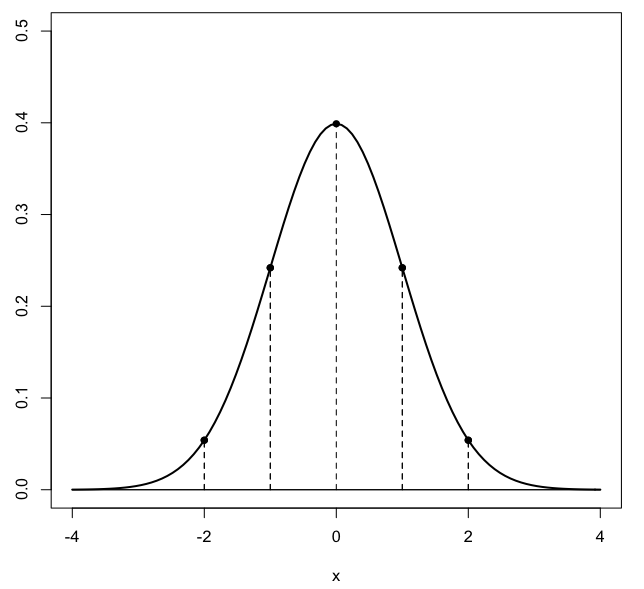
\includegraphics [scale=0.4] {gauss3.png} \end{center}

\title{Field of an infinite wire}
\date{}

\begin{document}
\maketitle
\Large

These are two classic problems:  find the electric field $\mathbf{E}$ for an infinite wire charged with density $\lambda$ or an infinite sheet charged with density $\sigma$ (positive charge).  Let's start with the wire.

The force between two charges is given by Coulomb's Law:
\[ \mathbf{F} = \frac{1}{4 \pi \epsilon_0} \ \frac{q_1 q_2}{r^2} \ \mathbf{\hat{e}}_r \]
while the field is the force on a unit test charge due to a given charge.
\[ \mathbf{E} = \frac{1}{4 \pi \epsilon_0} \ \frac{q}{r^2} \ \mathbf{\hat{e}}_r \]

\subsection*{infinite wire}
\begin{center} 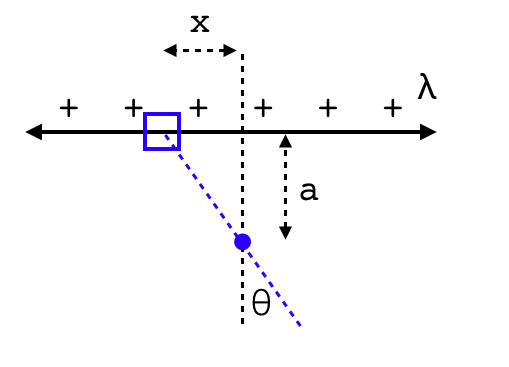
\includegraphics [scale=0.5] {charge_density1.png} \end{center}
Consider a point at a distance $a$ from the wire.  Call the nearest position on the wire $x=0$.  The force from a small element at position $x$ points radially away from the element.  

Break that force into two components, the component horizontal in the figure will be canceled by a component in the other direction from its counterpart at $-x$.  The vertical component is $F \cos \theta$.

Coulomb says that
\[ E = \frac{q}{4 \pi \epsilon_0} \frac{1}{r^2} \]
If the small element has width $dx$ and the density is $\lambda$, the total charge in that element is $\lambda dx$.  The distance from the element to the position we are evaluating is $\sqrt{x^2 + a^2}$.  So the small part of the electric field is
\[ dE = \frac{\lambda}{4 \pi \epsilon_0} \frac{dx}{(a^2 + x^2)} \]

There is a further factor of $\cos \theta$ to account for the fact that only the vertical part of the force is not canceled.  In terms of $a$ and $x$:
\[ \cos \theta = \frac{a}{\sqrt{a^2 + x^2}} \]
\[ dE = \frac{\lambda a}{4 \pi \epsilon_0} \frac{dx}{(a^2 + x^2)^{3/2}} \]

To integrate this, we need a trig substitution.  Because of the $a^2 + x^2$, choose the tangent.  (Also, Shankar says, we will want to integrate to $\infty$ as a limit, so neither sine nor cosine will do).
\[ x/a = \tan \theta \]
\[ x = a \tan \theta \]
\[ dx = a \sec^2 \theta \ d \theta \]
We already have
\[ a/\sqrt{a^2 + x^2} = \cos \theta \]
\[ \frac{1}{(a^2 + x^2)^{3/2}} = \frac{\cos^3 \theta}{a^3} \]
Thus
\[ dE = \frac{\lambda a}{4 \pi \epsilon_0} a \sec^2 \theta \ \frac{\cos^3 \theta}{a^3} \ d \theta \]
\[ dE = \frac{\lambda}{4 \pi \epsilon_0 a} \cos \theta \ d \theta \]
\[ E = \int \frac{\lambda}{4 \pi \epsilon_0 a} \cos \theta \ d \theta \]
\[ = \frac{\lambda}{4 \pi \epsilon_0 a} \ \sin \theta \]

The limits require care.    The original limits on $x$ were (for an infinite wire) $x = -\infty \rightarrow \infty$.  Now $x = \tan \theta$, so $\theta = -\pi/2 \rightarrow \pi/2$.  Evaluating $\sin \theta$ between those limits we get $1 - -1 = 2$.
\[ E = \frac{\lambda}{2 \pi \epsilon_0 a} \]

The field falls off like $1/a$ rather than $1/a^2$.  We visualize the electric field lines as being perpendicular to the wire.  If we take a cross-section in the perpendicular plane, the field lines spread like $1$ over the distance.  It is a one-dimensional spreading.

We can get the same result using Gauss's Law.  We haven't introduced it properly yet, but just state it here:

\[ \int_S \mathbf{E} \cdot \mathbf{r} = \frac{Q}{\epsilon_0} \]

The flux of the electric field across a closed surface is equal to the charge enclosed $Q$ times the constant $1/\epsilon_0$, which is about $9 \times 10^9$.

Surround a section of wire of length $L$ with a cylindrical Gaussian surface.  

\begin{center} 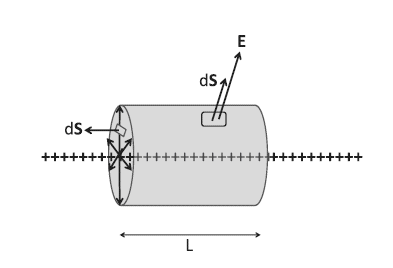
\includegraphics [scale=0.5] {gauss_wire.png} \end{center}

The amount of charge enclosed is $\lambda L$.  Gauss says

\[ \int_S \mathbf{E} \cdot \mathbf{r} = \frac{Q}{\epsilon_0} =  \frac{\lambda L}{\epsilon_0} \]

By symmetry, the field is radial, and so the dot product with the surface elements on the ends of the cylinder is zero.  The dot product with the surface elements on the curved part is just $E \ dS$ so the whole integral is

\[ \int_S \mathbf{E} \cdot \mathbf{dS} = E \int dS = E \ 2 \pi a L \]
\[  E \ 2 \pi a L =  \frac{\lambda L}{\epsilon_0} \]
\[ E = \frac{\lambda}{2 \pi a \epsilon_0} \]
and that matches what we had before.

\end{document}  